\documentclass{article}
\usepackage{listings}
\usepackage[utf8]{inputenc}
\usepackage{graphicx}
\renewcommand{\figurename}{Figura}
\usepackage{mathtools}
\usepackage{hyperref}
\usepackage[spanish]{babel}

\title{Informe de Estadística en Física Experimental: Guía 3 y 4}
\author{Andr\'es Babino}

\begin{document}
\maketitle
\section{Introducción}
El lenguaje utilizado para programar todas los ítems fue Python.
El código utilizado para generar los datos, gráficos y este mismo informe fue controlado con git, tiene licencia MIT y está almacenado en \url{https://github.com/ababino/efe}.

\section{Guía 3, Ejercicio 4, Ítem b}
En el gráfico de la figura \ref{fig:ej4b} se muestra la superposición de la distribución de Cauchy y la suma de dos Gaussianas.
Para x suficientemente chicos se ve que hay un acuerdo entre las dos distribucíones. 
Cuando $|x|$ es mayor a $6$ las colas gaussianas ya son menos pesadas que la de la disribución de Cauchy.


\begin{figure}
\centering
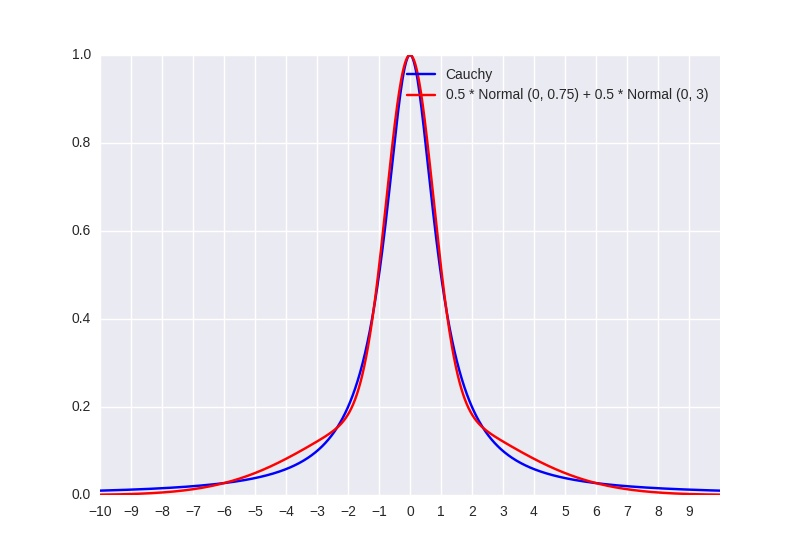
\includegraphics[width=0.75\textwidth]{ej4b.jpg}
\caption[]{Comparación entre la distribución de Cauchy y la suma de dos Gaussianas.}
\label{fig:ej4b}
\end{figure}

\section{Guía 3, Ejercicio 9, Ítem b}
$$f (x) = U(0, 1)$$
$$ g(y) = \lambda e^(-\lambda y)$$
$$g(y) \frac{dy}{dx} dx= f(x) dx $$

$$\lambda e^(-\lambda y) \frac{dy}{dx} = 1 $$

$$ y = -\frac{1}{\lambda} ln(1-x)$$

\begin{figure}
\centering
\includegraphics[width=0.75\textwidth]{ej9b.jpg}
\caption[]{}
\label{fig:ej9b}
\end{figure}

\section{Guía 4, Ejercicio 10}

\subsection{Ítem a}
$$f(r, \theta, \phi) = A \rho(r) $$
$$A = \frac{1}{\int_0^1 \int_0^{2\pi} \int_0^{\pi}\rho(r) sen(\theta) r^2 d\phi d\theta dr} $$
$$A = \frac{1}{\rho_0 \pi (4 - \pi)} $$

$$f(r, \theta, \phi) = \frac{1}{\pi (4 - \pi)} \frac{1}{1 + r^2} $$

\subsection{Ítem b}

$$f(r) = \int_0^{2\pi}\int_0^{\pi} f(r, \theta, \phi) sen(\theta) r^2 d\theta d\phi$$
$$f(r) = \frac{4 r^2}{(4 - \pi) (1 + r^2)}$$

$$f(\theta) = \int_0^1 \int_0^{2\pi}  f(r, \theta, \phi) sen(\theta) r^2 d\phi dr$$
$$f(\theta) = \frac{1}{2} sen(\theta)$$

$$f(\phi) = \int_0^1 \int_0^{\pi}  f(r, \theta, \phi) sen(\theta) r^2 d\theta dr$$
$$f(\theta) = \frac{1}{2\pi}$$

\subsection{Ítem c}

\begin{figure}
\centering
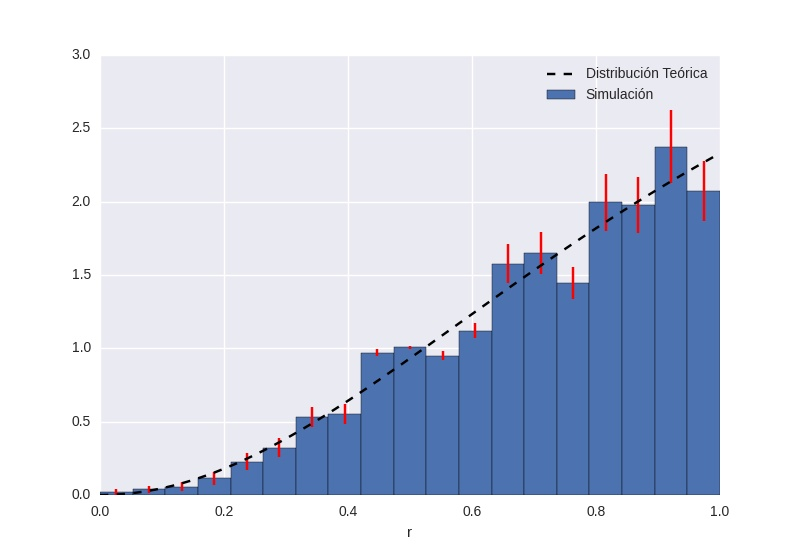
\includegraphics[width=0.75\textwidth]{g4ej10_r.jpg}
\caption[]{}
\label{fig:g4ej10_r}
\end{figure}

\begin{figure}
\centering
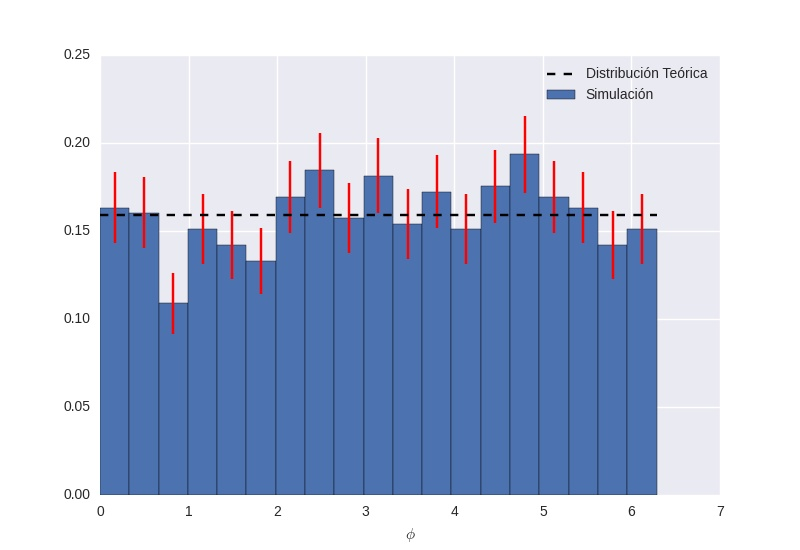
\includegraphics[width=0.75\textwidth]{g4ej10_phi.jpg}
\caption[]{}
\label{fig:g4ej10_phi}
\end{figure}

\begin{figure}
\centering
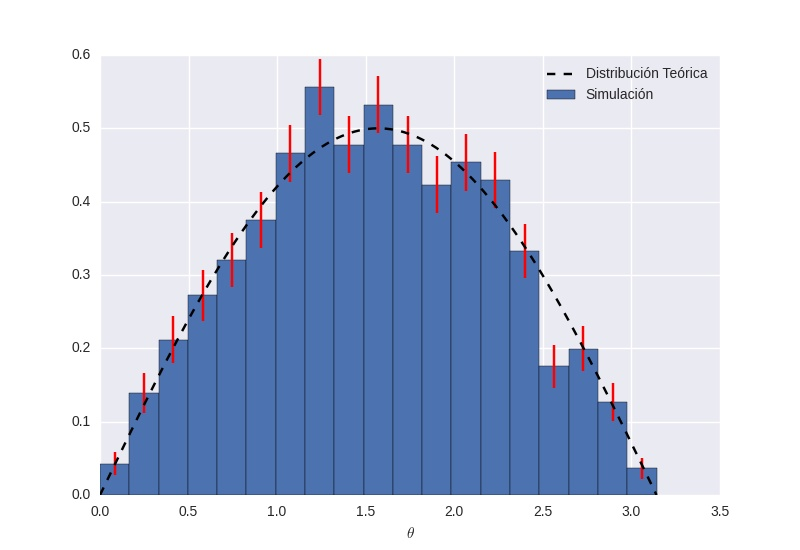
\includegraphics[width=0.75\textwidth]{g4ej10_theta.jpg}
\caption[]{}
\label{fig:g4ej10_theta}
\end{figure}


\end{document}
